\chapter{R (Part I: Basics)} \label{ch:r1}

This chapter and the sequential chapters introduce R language, a widely used programming language for data mining and visualization. 

This chapter focuses on the fundamental setup and basic operations such as the installation of R and RStudio, basic data types, vector and data frame manipulation, and finally basic visualization methods. Chapter \ref{ch:r2} introduces advanced data analysis skills and tools. Finally, Chapter \ref{ch:r3} put things into practice to solve actual problems.

\section{R and RStudio Installation} \label{ch:r1:sec:rinstallation}

\textit{R} is a programming language for statistical computing and visualization. It is widely used among statisticians and data miners for developing statistical software and carrying out data analysis. R is free and can be downloaded from \cite{r}, from which more details about R can also be found.

\textit{RStudio}, also known as \textit{Posit}, is an IDE widely used for R programming and testing. RStudio IDE is open-source and free of charge for personal use. It can be downloaded from \cite{rstudio}.

Download R and RStudio from the aforementioned web sites, and install them following the instructions.

\section{R Packages Management} \label{ch:r1:sec:rpackage}

R uses packages (sometimes known as libraries) to boost its capability. R packages, both built-in and third-party, provide powerful features for data analysis and visualization. Some packages may also come with demonstrative sample data frames. The packages can be published and shared online. CRAN is by far the most popular platform to store and share R packages.

\subsection{Manage Packages with Built-in Functions}

There are a number of default packages that come along with R and they do not need separate installation. Only third-party packages need additional installation. To install or remove a package, use
\begin{lstlisting}
install.packages("<package>")
remove.packages("<package>")
\end{lstlisting}
respectively. For example,
\begin{lstlisting}
install.packages("pacman")
\end{lstlisting}

To load a package, both default and third-party, use
\begin{lstlisting}
library(<package>)
\end{lstlisting}
For example
\begin{lstlisting}
library(pacman)
\end{lstlisting}
After loading a package, the data frames and functions defined in that package can be used normally. Alternatively, use prefix \verb|<package>::<function>|, \verb|<package>::<dataframe>| to call the functions and data frames defined in a package without loading it. The later approach can become inconvenient when the function or data frame is used frequently. 

To unload a package, use
\begin{lstlisting}
detach("package:<package>", unload = TRUE)
\end{lstlisting}
For example,
\begin{lstlisting}
detach("package:pacman", unload = TRUE)
\end{lstlisting}

\subsection{Manage Packages with Third-Party Packages}

There are third-party packages that provide package management functions, for example \verb|pacman|. With \verb|pacman| installed and loaded, use the following commands to install, load and unload packages respectively.
\begin{lstlisting}
p_install(<package>, ...) # install
p_load(<package>, ...) # load (if not installed, also install)
p_unload(<package>, ...) # unload
p_unload(all) # unload all
\end{lstlisting}
Assume that \verb|pacman| is already installed. An example of using \verb|pacman| to load packages are given as follows.
\begin{lstlisting}
pacman::p_load(
	pacman, # package management
	dplyr, # data manipulation
	GGally, # data visualization
	ggplot2, # data visualization
	ggthemes, # data visualization
	ggvis, # data visualization
	httr, # url and http
	lubridate, # date and time manipulation
	plotly, # data visualization
	rio, # io
	rmarkdown, # documentation
	shiny, # web apps development
	stringr, # string operation
	tidyr # data tidying
)
\end{lstlisting}
The above command can be executed without loading \verb|pacman| in advance since \verb|pacman::p_load()| prefix is used. The listed packages are commonly used in R projects, and a brief explanation to them is given as comments in the above demo. 

\subsection{Manage Packages with RStudio IDE}

RStudio provides a graphical interface to manage packages as shown in Fig. \ref{ch:r1:fig:rstudio_package_management}. A package can be loaded or unloaded simply by checking and unchecking the package.
\begin{figure}
\centering
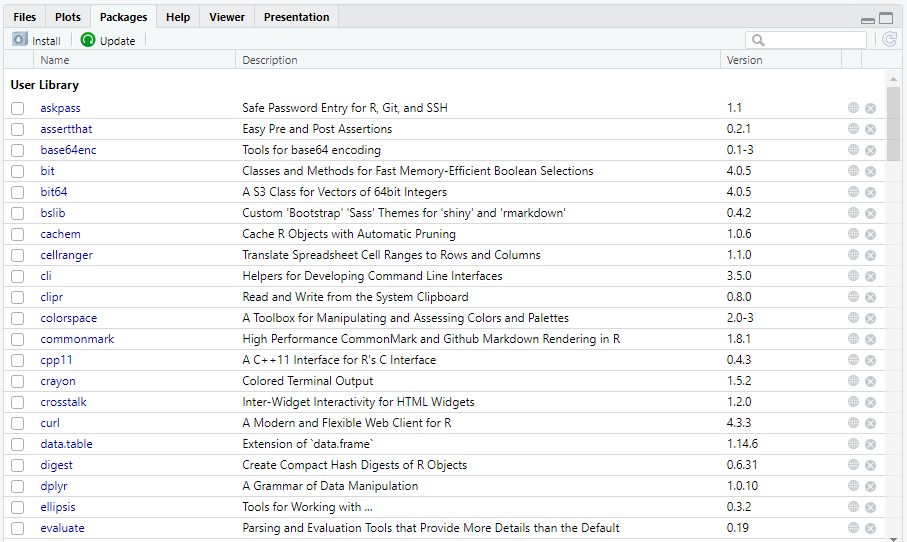
\includegraphics[width=350pt]{chapters/ch-r/figures/rstudio_package_management.png}
\caption{RStudio's graphical interface for package management.} \label{ch:r1:fig:rstudio_package_management}
\end{figure}

\section{Basic Syntax} \label{ch:r1:sec:rprogramming}

This section introduces the basic syntax and commonly used data types of R programming.

It is worth mentioning in the beginning that R is case sensitive. Use \verb|#| to lead a comment. In the console, use \verb|print(<variable>)| or simply type the name of the variable to print the value of a variable to the console. Use \verb|?<function>|, \verb|?<dataframe>| to access the manual for a function or data frame.

As a quick demonstrative example, the following is a small piece of code written in R. It generates generalized $t$-distribution noise and save the noise samples into a local CSV file.
\begin{lstlisting}
# Read parameters
generate_sgt_parameters <- read.csv('generate_sgt_parameters.csv', header = FALSE)
sgt_mu <- generate_sgt_parameters[,1]
sgt_sigma <- generate_sgt_parameters[,2]
sgt_lambda <- generate_sgt_parameters[,3]
sgt_p <- generate_sgt_parameters[,4]
sgt_q <- generate_sgt_parameters[,5]
sgt_n <- generate_sgt_parameters[,6]
sgt_seed <- generate_sgt_parameters[,7]

# Generate pseudo random numbers
library('optimx')
library('numDeriv')
library('sgt')
set.seed(sgt_seed)
x = rsgt(n = sgt_n, mu = sgt_mu, sigma = sgt_sigma, lambda = sgt_lambda, p = sgt_p, q = sgt_q, mean.cent = TRUE, var.adj = FALSE)

# Write data
write.table(x, 'generate_sgt_data.csv', sep=",", row.names = FALSE, col.names=FALSE)
\end{lstlisting}

\subsection{Data Types}

R supports many data types. Commonly used data types are summarized in Table \ref{ch:r1:tab:datatype}, where notice that \verb|<-| is used to assign a value to a variable. Use \verb|typeof()| to check the type of a variable. Alternatively, use \verb|is.numeric()|, \verb|is.integer()|, \verb|is.double()|, \verb|is.character()|, etc., to check whether a variable belongs to a particular data type.
\begin{table}
  \centering \caption{Commonly used data types.}\label{ch:r1:tab:datatype}
  \begin{tabularx}{\textwidth}{llX}
    \hline
    Data Type & Syntax (Example) & Description \\ \hline
    integer & \verb|n <- 2L| & An integer. Define an integer by a value followed by \verb|L|. \\
    double & \verb|x <- 2| & An double float value. \\
    complex & \verb|z <- 3+2i| & A complex value. \\
    character & \verb|a <- "a"| & A character or a string. \\
    logical & \verb|q <- T| & A boolean value. Use \verb|T|, \verb|TRUE| and \verb|F|, \verb|FALSE| to represent true and false respectively. \\
    \hline
  \end{tabularx}
\end{table}

Examples of assigning variables and checking their types are given as follows. Notice that \verb|>| is the prompt indicating that the commands are executed in a console.
\begin{lstlisting}
> n <- 2L
> typeof(n)
[1] "integer"

> x <- 2
> typeof(x)
[1] "double"

> z <- 3+2i
> typeof(z)
[1] "complex"

> a <- "h"
> typeof(a)
[1] "character"

> q <- T
> typeof(q)
[1] "logical"
\end{lstlisting}

To transform data from one type to another, use \verb|as.<datatype>()|. Examples of transforming data types are given as follows.
\begin{lstlisting}
> n1 <- as.integer(2)
> typeof(n1)
[1] "integer"

> n2 <- as.integer("2")
> typeof(n2)
[1] "integer"

> x1 <- as.double(2L)
> typeof(x1)
[1] "double"

> x2 <- as.double("2")
> typeof(x2)
[1] "double"

> z1 <- as.complex("3+2i")
> typeof(z1)
[1] "complex"

> a1 <- as.character(2L)
> typeof(a1)
[1] "character"

> a2 <- as.character(2)
> typeof(a2)
[1] "character"
\end{lstlisting}

R supports arithmetic calculations of variables, including \verb|+|, \verb|-|, \verb|*|, \verb|/|, \verb|%/%| (integer division), \verb|%%| (modulus) and \verb|^| (exponential). Examples of arithmetic calculations are given as follows.
\begin{lstlisting}
> a <- 16
> b <- 3
> add <- a + b
> sub <- a - b
> multi <- a * b
> division <- a / b
> int_division <- a %/% b
> modulus <- a %% b
> exponent <- a ^ b
> add
[1] 19
> sub
[1] 13
> multi
[1] 48
> division
[1] 5.333333
> int_division
[1] 5
> modulus
[1] 1
> exponent
[1] 4096
\end{lstlisting}

R uses built-in and third-party functions which extend its capability. There is a rich set of functions for numerical calculations, string operations, probability calculations and statistics analysis. Some of them are summarized in Tables \ref{ch:r1:tab:numericalcalculation}, \ref{ch:r1:tab:logicalcomparison}, \ref{ch:r1:tab:stringoperation}, \ref{ch:r1:tab:probabilityfunction} and \ref{ch:r1:tab:statisticsfunction}.

\begin{table}
  \centering \caption{Numerical calculations.}\label{ch:r1:tab:numericalcalculation}
  \begin{tabularx}{\textwidth}{lX}
    \hline
    Syntax & Description \\ \hline
    \verb|abs(x)| & Absolute value. \\
    \verb|sqrt(x)| & Square root. \\
    \verb|ceiling(x)| & Smallest larger/equal integer. \\
    \verb|floor(x)| & Largest smaller/equal integer. \\
    \verb|trunc(x)| & Integer part of a variable. \\
    \verb|round(x, n=0)| & Round to $n$ digit after decimal. \\
    \verb|sin(x)| & Trigonometric sin function. \\
    \verb|cos(x)| & Trigonometric cos function. \\
    \verb|tan(x)| & Trigonometric tan function. \\
    \verb|log(x)| & Natural logarithm. \\
    \verb|log10(x)| & Common logarithm. \\
    \verb|exp(x)| & Exponent. \\
    \hline
  \end{tabularx}
\end{table}

\begin{table}
  \centering \caption{Logical comparisons.}\label{ch:r1:tab:logicalcomparison}
  \begin{tabularx}{\textwidth}{lX}
    \hline
    Syntax & Description \\ \hline
    \verb|x == y| & Equal. \\
    \verb|x != y| & Not equal. \\
    \verb|x > y|, \verb|x < y| & Greater than; less than. \\
    \verb|x >= y|, \verb|x <= y| & Greater than or equal to; less than or equal to. \\
    \verb|!x| & Not. \\
    \verb|x & y| & And. \\
    \verb$x | y$ & Or. \\
    \verb|isTRUE(x)| & Is true. \\
    \hline
  \end{tabularx}
\end{table}

\begin{table}
  \centering \caption{String operations.}\label{ch:r1:tab:stringoperation}
  \begin{tabularx}{\textwidth}{lX}
    \hline
    Syntax & Description \\ \hline
    \verb|substr(s, n1, n2)| & Segment of a string, from the $n_1$-th character to $n_2$-th character, both characters included. The index starts from $1$ instead of $0$. \\
    \verb|grep(p, s)| & Searching for a pattern in a string. \\
    \verb|sub(s1, s2, s)| & Find and replace patterns in a string. \\
    \verb|paste(s1, s2, ..., p="")| & Concatenate strings. \\
    \verb|strsplit(s, p)| & Split a string. \\
    \verb|tolower(s)| & Convert to lower case. \\
    \verb|toupper(s)| & Convert to upper case. \\
    \hline
  \end{tabularx}
\end{table}

\begin{table}
	\centering \caption{Probability related operations.}\label{ch:r1:tab:probabilityfunction}
	\begin{tabularx}{\textwidth}{lX}
		\hline
		Syntax & Description \\ \hline
		\verb|dnorm(x, m=0, std=1)| & Calculate the PDF of Gaussian distribution. \\
		\verb|pnorm(x, m=0, std=1)| & Calculate the CDF of Gaussian distribution. \\
		\verb|qnorm(x, m=0, std=1)| & Inverse function of \verb|pnorm()|. \\
		\verb|rnorm(n, m=0, std=1)| & Generate Gaussian distribution samples. \\
		\verb|dbinom(n, size, p)| & Calculate the probability of a binominal distribution. \\
		\verb|pbinom(n, size, p)| & Calculate the comulative probability of a binominal distribution. \\
		\verb|qbinom(x, size, p)| & Inverse function of \verb|pbinom()|. \\
		\verb|rbinom(n, size, p)| & Generate binominal distribution samples. \\
		\verb|dpois(x, lambda)| & Calculate the probability of a Poisson distribution. \\
		\verb|ppois(n, lambda)| & Calculate the comulative probability of a Poisson distribution. \\
		\verb|qpois(x, lambda)| & Inverse function of \verb|ppois()|. \\
		\verb|rpois(n, lambda)| & Generate Poisson distribution samples. \\
		\verb|dunif(x, min=0, max=1)| & Calculate the PDF of uniform distribution. \\
		\verb|punif(x, min=0, max=1)| & Calculate the CDF of uniform distribution. \\
		\verb|qunif(x, min=0, max=1)| & Inverse function of \verb|punif()|. \\
		\verb|runif(n, min=0, max=1)| & Generate uniform distribution samples. \\
		\hline
	\end{tabularx}
\end{table}

\begin{table}
	\centering \caption{Statistics related functions.}\label{ch:r1:tab:statisticsfunction}
	\begin{tabularx}{\textwidth}{lX}
		\hline
		Syntax & Description \\ \hline
		\verb|mean(l)| & Mean. \\
		\verb|sd(l)| & Standard deviation. \\
		\verb|median(l)| & Median. \\
		\verb|range(l)| & Minimum and maximum. \\
		\verb|min(l)| & Minimum. \\
		\verb|max(l)| & Maximum. \\
		\verb|sum(l)| & Sum \\
		\hline
	\end{tabularx}
\end{table}

\subsection{Conditionals and Loops}

The \verb|if| statement syntax is given as follows.
\begin{lstlisting}
if(<condition>){
	<command>
} else if(<condition>){
	<command>
} else{
	<command>
}
\end{lstlisting}
An example of using \verb|if| statement is givne below.
\begin{lstlisting}
> x <- rnorm(1)
> if(x > 0){
	+   y <- x
	+ } else if(x < 0){
	+   y <- -x
	+ } else{
	+   y <- 0
	+ }
> print(x)
[1] -1.981445
> print(y)
[1] 1.981445
\end{lstlisting}
where \verb|+| indicates the splitting of commands in multiple lines in the console.

The \verb|for| loop syntax is given as follows.
\begin{lstlisting}
for(<variable> in <vector>){
	<command>
}
\end{lstlisting}
where \verb|<vector>| is a list of numbers or characters. Examples are given below.
\begin{lstlisting}
> for(i in 1:5){
	+     print(i)
	+ }
[1] 1
[1] 2
[1] 3
[1] 4
[1] 5

> for(i in c("a", "b", "c")){
	+     print(i)
	+ }
[1] "a"
[1] "b"
[1] "c"
\end{lstlisting}
where \verb|c()| defines a list from items. This command is widely used. More details will be introduced later.

The \verb|while| loop syntax is given as follows.
\begin{lstlisting}
while(<condition>){
    <command>
}
\end{lstlisting}
An example of using \verb|while| loop is given below.
\begin{lstlisting}
> counter <- 0
> while(counter < 5){
+     print(counter)
+     counter <- counter + 1
+ }
[1] 0
[1] 1
[1] 2
[1] 3
[1] 4
\end{lstlisting}


An example using the above to estimate the ratio of data of a standard normal distribution between $\pm 1$ is given below.
\begin{lstlisting}
> N <- 1000000
> counter <- 0
> for(i in rnorm(N)){
	+   if(-1 < i & i < 1){
		+     counter <- counter + 1
		+   }
	+ }
> answer <- counter / N # expected: 0.682689492
> print(answer)
[1] 0.682407
\end{lstlisting}

\subsection{User-Defined Functions}

Define a simple function as follows. Run the codes where the function is described before calling the function.
\begin{lstlisting}
<function-name> <- function(<input>[=<default>], ...){
	<command>
	[return(<variable>)]
}
\end{lstlisting}

\section{Vector and Matrix}

Vector and matrix are the fundamental forms using which R stores and processes data.

\subsection{Vector}

There are different types of vectors in R depending on the data type of the elements it stores. The commonly used vector types include numeric vector and character vector. All elements in a vector must have the same data type. When different data type values are stored in a vector, they will be transferred to the most general data type.

Notice that the index of a vector in R starts from 1 instead of 0. This is different from many other computer languages such as C/C++, JavaScript and Python.

Use the following syntax to create a vector.
\begin{lstlisting}
<vector> <- c(<value>, ...)
\end{lstlisting}
where \verb|<value>| can be single element or a vector. Nested vector is expanded. For example,
\begin{lstlisting}
> x <- c(1,2,3,4,5)
> x
[1] 1 2 3 4 5
> y <- c(c(1,2,3),4,5,6,7)
> y
[1] 1 2 3 4 5 6 7
> z = c(x, 1,2,3,4,5)
> z
[1] 1 2 3 4 5 1 2 3 4 5
> typeof(z)
[1] "double"
\end{lstlisting}
It is possible to assign names to each element as shown below.
\begin{lstlisting}
> v <- c(1, 2, 3, 4, 5)
> names(v) <- c("e1", "e2", "e3", "e4", "e5") 	
> print(v)
e1 e2 e3 e4 e5
1  2  3  4  5
\end{lstlisting}

Alternative ways to create a vector are given as follows. Use sequence to create a vector as follows.
\begin{lstlisting}
<vector> <- seq(<from>, <to>, <by=1>)
<vector> <- <from>:<to> # equivalent to seq() with by=1
\end{lstlisting}

Use replica to create a vector as follows.
\begin{lstlisting}
<vector> <- rep(<value>, <repeat>)
\end{lstlisting}
where \verb|<value>| can be a numeric number, a character, or a vector. For example,
\begin{lstlisting}
> l <- rep(c("a", "b", "cde"), 2)
> print(l)
[1] "a"   "b"   "cde" "a"   "b"   "cde"
\end{lstlisting}
Replica can also be used to create empty vector with \verb|rep(NA, n)|.

A character vector can also be created by splitting strings using \verb|strsplit()|. For example,
\begin{lstlisting}
> a <- "Hello World!"
> b <- strsplit(a, "")
> print(b)
[[1]]
[1] "H" "e" "l" "l" "o" " " "W" "o" "r" "l" "d" "!"
\end{lstlisting}

To access the element in a vector, use \verb|<vector>[<index>]| or \verb|<vector>["<name>"]|. Notice that the first element in a vector has the index of 1 instead of 0. The index can be an integer, or an integer vector. Examples are given below.
\begin{lstlisting}
> s <- c("a", "b", "c", "d", "e", "f", "g")
> s[1]
[1] "a"
> s[7]
[1] "g"
> s[2:5]
[1] "b" "c" "d" "e"
> s[c(1, 3, 5)]
[1] "a" "c" "e"
\end{lstlisting}
It is also possible to address an element by its name
\begin{lstlisting}
> v <- c(1, 2, 3, 4, 5)
> names(v) <- c("e1", "e2", "e3", "e4", "e5") 	
> print(v)
e1 e2 e3 e4 e5
1  2  3  4  5
> print(v[3])
e3
3
> print(v["e3"])
e3
3
\end{lstlisting}

Vectorization operation significantly speeds up the calculation comparing with looping over elements, hence is quite commonly seen in high-layer languages such as R and Python. Most numerical calculations, including \verb|+|, \verb|-|, \verb|*|, \verb|/|, \verb|%/%|, \verb|%%|, \verb|^|, support vectorization operation. Examples are given below.
\begin{lstlisting}
> a <- c(1,2,3,4,5)
> b <- c(5,4,3,2,1)
> a + b
[1] 6 6 6 6 6
> a - b
[1] -4 -2  0  2  4
> a * b
[1] 5 8 9 8 5
> a / b
[1] 0.2 0.5 1.0 2.0 5.0
> a %/% b
[1] 0 0 1 2 5
> a %% b
[1] 1 2 0 0 0
> a ^ b
[1]  1 16 27 16  5
\end{lstlisting}
It is also possible to apply logic operations using vectors. Examples are given below.
\begin{lstlisting}
> a <- c(1,2,3,4,5)
> b <- c(5,4,3,2,1)
> a < b
[1]  TRUE  TRUE FALSE FALSE FALSE
> a > b
[1] FALSE FALSE FALSE  TRUE  TRUE
> a == b
[1] FALSE FALSE  TRUE FALSE FALSE
\end{lstlisting}
When the sizes of the vectors are not consistent, the shorter vector will repeat and populate to align with the longer vector. Examples are given below.
\begin{lstlisting}
> a <- c(1,10)
> b <- c(1,2,3,4)
> a + b
[1]  2 12  4 14
> a - b
[1]  0  8 -2  6
> a * b
[1]  1 20  3 40
> a / b
[1] 1.0000000 5.0000000 0.3333333 2.5000000
> a %/% b
[1] 1 5 0 2
> a %% b
[1] 0 0 1 2
> a ^ b
[1]     1   100     1 10000
\end{lstlisting}

A vector can also be used as an input argument or output return of a function.

\subsection{Matrix}

Similar with vector, all elements in a matrix must have the consistent type. A demonstration of matrix indexing in R is shown in Fig. \ref{ch:r1:fig:r_table_demo}. Let the matrix be named \verb|A|. The elements in the matrix can be accessed by the name of the table followed by the index coordinates. For example, in the figure, \verb|A[1,1]| refers to the first element and \verb|A[4,6]| the last element. It is also possible to index an entire row or column. For example, use \verb|A[1,]| to represent the first row of the matrix.

\begin{figure}
	\centering
	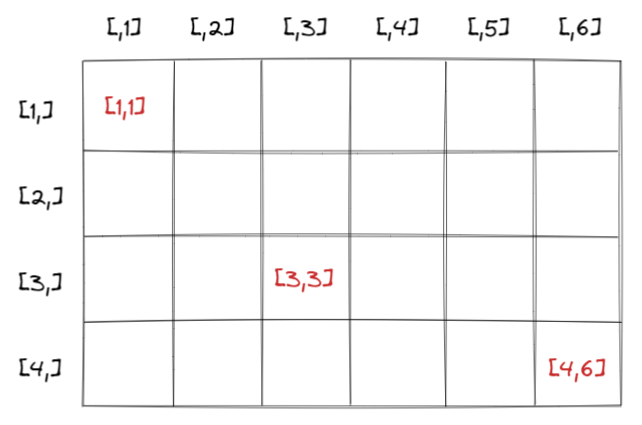
\includegraphics[width=250pt]{chapters/ch-r/figures/r_table_demo.png}
	\caption{A demonstration of a matrix in R.} \label{ch:r1:fig:r_table_demo}
\end{figure}

A matrix can be created from scratch by stacking rows as follows. First, create rows in the matrix. Then, use \verb|rbind()| to bind rows.
\begin{lstlisting}
# build rows
<row1> <- c(<value11>, ..., <value1n>)
...
<rowm> <- c(<valuem1>, ..., <valuemn>)
# build matrix
<matrix> <- rbind(<row1>, ..., <rowm>)
\end{lstlisting}

There are alternative ways, other than \verb|rbind()|, to create a matrix. For example, \verb|matrix()| convert a vector into a matrix. Similar with \verb|rbind()|, \verb|cbind()| binds the columns to form a matrix. Examples to create matrices using different methods are given below.
\begin{lstlisting}
> A <- matrix(1:9, 3, 3)
> print(A)
[,1] [,2] [,3]
[1,]    1    4    7
[2,]    2    5    8
[3,]    3    6    9
> B <- rbind(c(1, 4, 7), c(2, 5, 8), c(3, 6, 9))
> print(B)
[,1] [,2] [,3]
[1,]    1    4    7
[2,]    2    5    8
[3,]    3    6    9
> C <- cbind(c(1, 2, 3), c(4, 5, 6), c(7, 8, 9))
> print(C)
[,1] [,2] [,3]
[1,]    1    4    7
[2,]    2    5    8
[3,]    3    6    9
\end{lstlisting}

As illustrated earlier that \verb|names(<vector>)| can be used to view and assign names to elements in a vector, likewise \verb|rownames(<matrix>)| and \verb|colnames(<matrix>)| can be used to view and assign names to the rows and columns of a matrix. Examples are given below.
\begin{lstlisting}
> A <- matrix(1:9, 3, 3)
> colnames(A) <- c("col1", "col2", "col3")
> rownames(A) <- c("row1", "row2", "row3")
> A
col1 col2 col3
row1    1    4    7
row2    2    5    8
row3    3    6    9
> colnames(A)
[1] "col1" "col2" "col3"
> rownames(A)
[1] "row1" "row2" "row3"
> A[1,1]
[1] 1
> A["row1", "col1"]
[1] 1
> A[1,2]
[1] 4
> A["row1", "col2"]
[1] 4
\end{lstlisting}
To remove the names, simply assign \verb|NULL| to the name.

Vectorization operators are defined for matrix level as well. For example, for two matrices with the same shape, numerical operations such as  \verb|+|, \verb|-|, \verb|*|, \verb|/|, \verb|%/%|, \verb|%%| and \verb|^| can be used.

As introduced earlier, a matrix or a vector can be split and segmented to form a smaller matrix or vector. It is worth mentioning that when a single column or row is selected, R will automatically treated the return as a vector instead of a matrix. An example is given below. When a matrix downgrades to a vector, the row name (if it has only one row), or the column name (if it has only one column) will be removed.
\begin{lstlisting}
	> A <- matrix(1:9, 3, 3)
	> is.matrix(A)
	[1] TRUE
	> is.vector(A)
	[1] FALSE
	> is.matrix(A[1,])
	[1] FALSE
	> is.vector(A[1,])
	[1] TRUE
\end{lstlisting}

To get consistent results, when segmenting matrix to get a single row or column vector, deliberately ask R to not drop the matrix dimensions. This can be done as follows. By doing this, the names assigned to columns and rows preserve.
\begin{lstlisting}
	> A <- matrix(1:9, 3, 3)
	> is.matrix(A[1,,drop=F]) # select a row/column
	[1] TRUE
	> is.matrix(A[2,3,drop=F]) # select an element
	[1] TRUE
\end{lstlisting}

\subsection{Matrix Visualization Using \texttt{matplot()}}

R provides flexible and powerful data visualization tools, many of which more advanced than what is to be introduced in this section. This section introduces a simple matrix visualization function called \verb|matplot()|, which plots the columns of a matrix against each other.

To demonstrate \verb|matplot()|, consider the following example.
\begin{lstlisting}
professor <- c(1130, 1026, 893, 922, 776)
student <- c(2, 14, 24, 49, 46)
citation <- rbind(professor, student)
colnames(citation) <- c("2018", "2019", "2020", "2021", "2022")
rownames(citation) <- c("Professor", "Student")
print(citation)
citation.ratio <- citation
citation.ratio["Professor",] <- round(citation["Professor",] / mean(citation["Professor",]) * 100, 1)
citation.ratio["Student",] <- round(citation["Student",] / mean(citation["Student",]) * 100, 1)
print(citation.ratio)
matplot(
	2018:2022, # x axis
	t(citation.ratio), # y axis
	type="b", # line and point selection
	pch = 15:16, # point shape
	col = 1:2, # color
	xlab = "Year",
	ylab = "Citations Moving Ratio (%)"
)
legend("bottomright", inset = 0.01, legend = rownames(citation.ratio), pch = 15:16, col = 1:2, horiz = F)
\end{lstlisting}
where \verb|t()| used inside \verb|matplot()| calculates the transpose of a matrix. Save the above in a script and execute the code, to get the following Fig. \ref{ch:r1:fig:matplot_demo}.
\begin{figure}
	\centering
	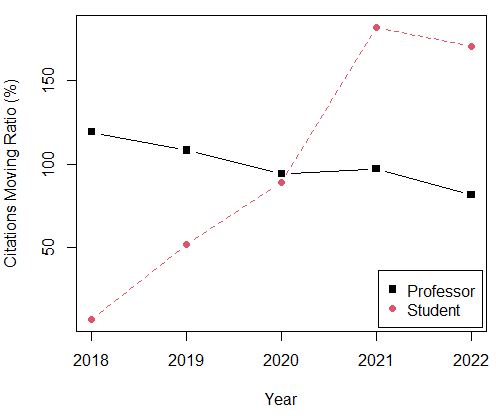
\includegraphics[width=250pt]{chapters/ch-r/figures/matplot_demo.png}
	\caption{A demonstration of using \texttt{matplot} to plot trends.} \label{ch:r1:fig:matplot_demo}
\end{figure}

Another example of analyzing the performance of players through a series of basketball games are given below.
\begin{lstlisting}
# generate table
player_name <- c("player1", "player2", "player3")
match_name <- c("match1", "match2", "match3", "match4", "match5", "match6", "match7", "match8", "match9", "match10")
penalty_attempt <- abs(matrix(round(rnorm(3*10, 5, 2)), 3, 10))
penalty_point <- abs(penalty_attempt - matrix(abs(round(rnorm(3*10, 1, 1))), 3, 10))
throw_attempt <- abs(matrix(round(rnorm(3*10, 15, 3)), 3, 10))
total_point <- abs(3*throw_attempt - abs(matrix(round(rnorm(3*10, 5, 1)), 3, 10))) + penalty_point
rownames(penalty_attempt) <- player_name
colnames(penalty_attempt) <- match_name
rownames(penalty_point) <- player_name
colnames(penalty_point) <- match_name
rownames(throw_attempt) <- player_name
colnames(throw_attempt) <- match_name
rownames(total_point) <- player_name
colnames(total_point) <- match_name

# claim function
myplot <- function(table, xlab, ylab){
    row_name = rownames(table)
    column_name = colnames(table)
    matplot(
    	1:length(column_name), # x axis
    	t(table), # y axis
    	type="b", # line and point selection
    	pch = 1:length(row_name), # point shape
    	col = 1:length(row_name), # color
    	xlab = xlab,
    	ylab = ylab
    )
    legend("bottomleft", inset = 0.01, legend = row_name, pch = 1:length(row_name), col = 1:length(row_name), horiz = F)
}

# plot
myplot(penalty_point / penalty_attempt, "match", "penalty success rate") # penalty successful rate
myplot((total_point - penalty_point) / throw_attempt, "match", "average gained point per throw") # average point gained per throw
\end{lstlisting}

The results of the above codes are given in Figs. \ref{ch:r1:fig:basket_exp1} and \ref{ch:r1:fig:basket_exp2}.

\begin{figure}
	\centering
	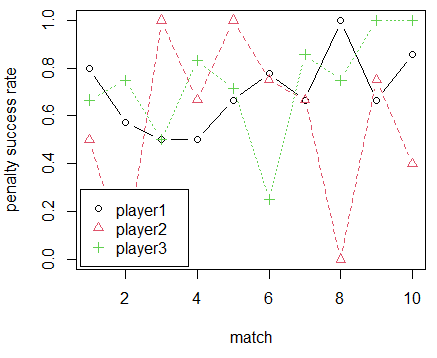
\includegraphics[width=250pt]{chapters/ch-r/figures/basket_exp1.png}
	\caption{Plot of penalty success rate of the 3 players in 10 matches.} \label{ch:r1:fig:basket_exp1}
\end{figure}

\begin{figure}
	\centering
	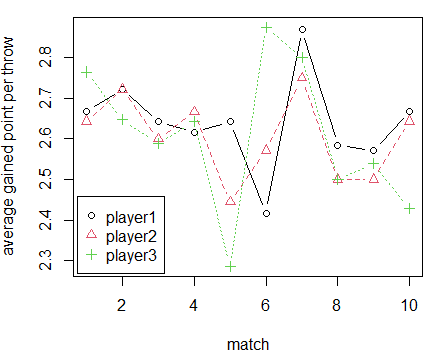
\includegraphics[width=250pt]{chapters/ch-r/figures/basket_exp2.png}
	\caption{Plot of average point gained per throw attempt for the 3 players in 10 matches.} \label{ch:r1:fig:basket_exp2}
\end{figure}

Notice that \verb|matplot()| is not widely used in practice comparing with the other visualization tools to be introduced in later sections.

\section{Data Frames} \label{ch:r1:sec:df}

Data frame, just like vector and matrix, is another data structure defined in R. Both matrix and data frame use tables to store data, but data frame does not require all data to have the same data type, which makes it more flexible and hence very widely used in R. Another difference between matrix and data frame is that data frame rows do not have names.

\subsection{Import Data into Data Frame}

Data frame can be created from scratch by concatenating columns just like matrix. However, in practice it is more common that a data frame is obtained by importing data from other data sources. Hence, data importing is introduced first and data concatenating will be introduced in a later section.

One of the most common sources of data is CSV files. R provides convenient functions to read data from CSV files into data frames. Use the following commands to import data from a CSV file into a data frame.

The following command pops up a separate window that allows the user to choose a CSV file manually.
\begin{lstlisting}
<data-frame> <- read.csv(file.choose()) # manual selection
\end{lstlisting}
The following commands import a specified CSV file.
\begin{lstlisting}
setwd("<directory>") # navigate to the directory of the csv file
<data-frame> <- read.csv("<csv-file>.csv")
\end{lstlisting}
where notice that \verb|getwd()| and \verb|setwd()| can be used to get and set current working directory respectively.

\subsection{Access Data in Data Frame}

There are a few ways to access an element in a data frame as shown below.
\begin{lstlisting}
<df>[<row_index>,<column_index>]
<df>[<row_index>,"<column_name>"]
<df>[,<column-name>][<row_index>]
<df>$<column_name>[<row_index>]
\end{lstlisting}
where the later two essentially adopt a 2-step precedure and
\begin{lstlisting}
<df>[, <column-name>]
<df>$<column-name>
\end{lstlisting}
are used to access the entire column in a data frame. Notice that different from a matrix, rows in data frame do not have names.

Table \ref{ch:r1:tab:dataframeexplore} summarizes the commonly used functions on date frames, such as checking its shape and data types.
\begin{table}
  \centering \caption{Commonly used commands for data frame exploration.}\label{ch:r1:tab:dataframeexplore}
  \begin{tabularx}{\textwidth}{lX}
    \hline
    Syntax (Example) & Description \\ \hline
    \verb|nrow(df)| & Number of rows. \\
    \verb|ncol(df)| & Number of columns. \\
    \verb|head(df, n=6L)| & Display the first few rows. \\
    \verb|tail(df, n=6L)| & Display the last few columns. \\
    \verb|str(df)| & A summary of the data frame, including the structure of each column. \\
    \verb|summary(df)| & A summary of the data frame, including some of its statistics features. \\
    \verb|levels(df$<column>)| & The level of the column. \\
    \hline
  \end{tabularx}
\end{table}
Examples of applying these functions to \verb|iris| data frame from the built-in \verb|datasets| package are given below.
\begin{lstlisting}
> library(datasets)
> nrow(iris)
[1] 150
> ncol(iris)
[1] 5
> head(iris)
  Sepal.Length Sepal.Width Petal.Length Petal.Width Species
1          5.1         3.5          1.4         0.2  setosa
2          4.9         3.0          1.4         0.2  setosa
3          4.7         3.2          1.3         0.2  setosa
4          4.6         3.1          1.5         0.2  setosa
5          5.0         3.6          1.4         0.2  setosa
6          5.4         3.9          1.7         0.4  setosa
> tail(iris)
    Sepal.Length Sepal.Width Petal.Length Petal.Width   Species
145          6.7         3.3          5.7         2.5 virginica
146          6.7         3.0          5.2         2.3 virginica
147          6.3         2.5          5.0         1.9 virginica
148          6.5         3.0          5.2         2.0 virginica
149          6.2         3.4          5.4         2.3 virginica
150          5.9         3.0          5.1         1.8 virginica
> str(iris)
'data.frame':	150 obs. of  5 variables:
 $ Sepal.Length: num  5.1 4.9 4.7 4.6 5 5.4 4.6 5 4.4 4.9 ...
 $ Sepal.Width : num  3.5 3 3.2 3.1 3.6 3.9 3.4 3.4 2.9 3.1 ...
 $ Petal.Length: num  1.4 1.4 1.3 1.5 1.4 1.7 1.4 1.5 1.4 1.5 ...
 $ Petal.Width : num  0.2 0.2 0.2 0.2 0.2 0.4 0.3 0.2 0.2 0.1 ...
 $ Species     : Factor w/ 3 levels "setosa","versicolor",..: 1 1 1 1 1 1 1 1 1 1 ...
> summary(iris)
  Sepal.Length    Sepal.Width     Petal.Length    Petal.Width          Species
 Min.   :4.300   Min.   :2.000   Min.   :1.000   Min.   :0.100   setosa    :50
 1st Qu.:5.100   1st Qu.:2.800   1st Qu.:1.600   1st Qu.:0.300   versicolor:50
 Median :5.800   Median :3.000   Median :4.350   Median :1.300   virginica :50
 Mean   :5.843   Mean   :3.057   Mean   :3.758   Mean   :1.199
 3rd Qu.:6.400   3rd Qu.:3.300   3rd Qu.:5.100   3rd Qu.:1.800
 Max.   :7.900   Max.   :4.400   Max.   :6.900   Max.   :2.500
> levels(iris$Species) # only works for discrete-value columns
[1] "setosa"     "versicolor" "virginica"
\end{lstlisting}

Data frame segmentation works similarly with matrix. A segmentation of multiple rows and columns of a data frame is also a data frame. Notice that when a single column is segmented, the result will be a vector by default, and \verb|drop=F| can be used to preserve data frame structure. An example is given below.
\begin{lstlisting}
> library(datasets)
> print(iris[1:5,])
  Sepal.Length Sepal.Width Petal.Length Petal.Width Species
1          5.1         3.5          1.4         0.2  setosa
2          4.9         3.0          1.4         0.2  setosa
3          4.7         3.2          1.3         0.2  setosa
4          4.6         3.1          1.5         0.2  setosa
5          5.0         3.6          1.4         0.2  setosa
> print(iris[1,])
  Sepal.Length Sepal.Width Petal.Length Petal.Width Species
1          5.1         3.5          1.4         0.2  setosa
> is.data.frame(iris[1,])
[1] TRUE
> print(iris[,1]) # equivalent to print(iris@Sepal.Length)
  [1] 5.1 4.9 4.7 4.6 5.0 5.4 4.6 5.0 4.4 4.9 5.4 4.8 4.8 4.3 5.8 5.7 5.4 5.1 5.7 5.1 5.4 5.1 4.6 5.1
 [25] 4.8 5.0 5.0 5.2 5.2 4.7 4.8 5.4 5.2 5.5 4.9 5.0 5.5 4.9 4.4 5.1 5.0 4.5 4.4 5.0 5.1 4.8 5.1 4.6
 [49] 5.3 5.0 7.0 6.4 6.9 5.5 6.5 5.7 6.3 4.9 6.6 5.2 5.0 5.9 6.0 6.1 5.6 6.7 5.6 5.8 6.2 5.6 5.9 6.1
 [73] 6.3 6.1 6.4 6.6 6.8 6.7 6.0 5.7 5.5 5.5 5.8 6.0 5.4 6.0 6.7 6.3 5.6 5.5 5.5 6.1 5.8 5.0 5.6 5.7
 [97] 5.7 6.2 5.1 5.7 6.3 5.8 7.1 6.3 6.5 7.6 4.9 7.3 6.7 7.2 6.5 6.4 6.8 5.7 5.8 6.4 6.5 7.7 7.7 6.0
[121] 6.9 5.6 7.7 6.3 6.7 7.2 6.2 6.1 6.4 7.2 7.4 7.9 6.4 6.3 6.1 7.7 6.3 6.4 6.0 6.9 6.7 6.9 5.8 6.8
[145] 6.7 6.7 6.3 6.5 6.2 5.9
> is.data.frame(iris[,1])
[1] FALSE
> print(iris[,1,drop=F]) # preserve data frame
    Sepal.Length
1            5.1
2            4.9
3            4.7
... # WRAPPED # ...
148          6.5
149          6.2
150          5.9
> is.data.frame(iris[,1,drop=F])
[1] TRUE
\end{lstlisting}

To add a new column to an existing data frame, just assign values to a new column name as follows.
\begin{lstlisting}
<df>$<new-column> <- <vector>
\end{lstlisting}
if there is a mismatch in size, \verb|<vector>| will be cycled. To remove a column, assign \verb|NULL| to the column as follows.
\begin{lstlisting}
<df>$<column> <- NULL
\end{lstlisting}

\subsection{Filter Data from Data Frame}

Filtering allows selecting rows from a data frame that meet specific criteria. A true-false vector can be used as a filter as follows.
\begin{lstlisting}
<filter-name> <- <true-false-vector> # use true-false vector as filter
<df>[filter,] # implement filter on data frame
\end{lstlisting}
An example is given below.
\begin{lstlisting}
> library(datasets)
> filter <- iris$Sepal.Length >= 7
> print(iris[filter,])
    Sepal.Length Sepal.Width Petal.Length Petal.Width    Species
51           7.0         3.2          4.7         1.4 versicolor
103          7.1         3.0          5.9         2.1  virginica
106          7.6         3.0          6.6         2.1  virginica
108          7.3         2.9          6.3         1.8  virginica
110          7.2         3.6          6.1         2.5  virginica
118          7.7         3.8          6.7         2.2  virginica
119          7.7         2.6          6.9         2.3  virginica
123          7.7         2.8          6.7         2.0  virginica
126          7.2         3.2          6.0         1.8  virginica
130          7.2         3.0          5.8         1.6  virginica
131          7.4         2.8          6.1         1.9  virginica
132          7.9         3.8          6.4         2.0  virginica
136          7.7         3.0          6.1         2.3  virginica
> filter <- iris$Sepal.Length >= 7 & iris$Sepal.Width >= 3.5
> print(iris[filter,])
    Sepal.Length Sepal.Width Petal.Length Petal.Width   Species
110          7.2         3.6          6.1         2.5 virginica
118          7.7         3.8          6.7         2.2 virginica
132          7.9         3.8          6.4         2.0 virginica
\end{lstlisting}
As shown above, it is possible to use \verb|&|, \verb$|$ to form a more complex filter. The commands can be merged together as follows.
\begin{lstlisting}
> print(iris[iris$Sepal.Length >= 7,])
    Sepal.Length Sepal.Width Petal.Length Petal.Width    Species
51           7.0         3.2          4.7         1.4 versicolor
103          7.1         3.0          5.9         2.1  virginica
106          7.6         3.0          6.6         2.1  virginica
108          7.3         2.9          6.3         1.8  virginica
110          7.2         3.6          6.1         2.5  virginica
118          7.7         3.8          6.7         2.2  virginica
119          7.7         2.6          6.9         2.3  virginica
123          7.7         2.8          6.7         2.0  virginica
126          7.2         3.2          6.0         1.8  virginica
130          7.2         3.0          5.8         1.6  virginica
131          7.4         2.8          6.1         1.9  virginica
132          7.9         3.8          6.4         2.0  virginica
136          7.7         3.0          6.1         2.3  virginica
> nrow(iris[iris$Sepal.Length >= 7,]) # count the result number
[1] 13
\end{lstlisting}

\subsection{Create Data Frames}

So far we have been importing data or using existing \verb|iris| data frame in the well-defined library \verb|datasets| in the case study. Data frame can also be created from scratch using columns of data. To create a new data frame from scratch, use function \verb|data.frame()| as follows.
\begin{lstlisting}
<df> <- data.frame(<vector>, ...) # add a column
colnames(<df>) <- c("<column-name>", ...)
\end{lstlisting}
or
\begin{lstlisting}
<df> <- data.frame(<column-name> = <vector>, ...)
\end{lstlisting}

An example is given below, where a data frame of mortgage price at 3 types of areas, namely ``CBD'', ``city'' and ``suburbs'', are is created. Arbitrary data is used.
\begin{lstlisting}
# create data frame
vec_region <- c(rep("CBD", 100), rep("City", 100), rep("Suburbs", 100))
vec_size_cbd <- rnorm(100, 75, 10)
vec_size_city <- rnorm(100, 100, 15)
vec_size_suburbs <- rnorm(100, 150, 25)
vec_size = c(vec_size_cbd, vec_size_city, vec_size_suburbs)
vec_price_cbd <- vec_size_cbd*rnorm(100, 12500, 2500)
vec_price_city <- vec_size_city*rnorm(100, 7500, 1000)
vec_price_suburbs <- vec_size_suburbs*rnorm(100, 5000, 1000)
vec_price <- c(vec_price_cbd, vec_price_city, vec_price_suburbs)
mortgage_price <- data.frame(Region = vec_region, Size = vec_size, Price = vec_price)
rm(vec_region, vec_size_cbd, vec_size_city, vec_size_suburbs, vec_size, vec_price_cbd, vec_price_city, vec_price_suburbs, vec_price)
\end{lstlisting}
which gives the following result
\begin{lstlisting}
> head(mortgage_price)
  Region     Size     Price
1    CBD 81.84889 1154873.0
2    CBD 77.78946  831468.7
3    CBD 84.60477  735265.2
4    CBD 62.42625  829977.5
5    CBD 65.42723  933851.3
6    CBD 82.43867 1208589.0
\end{lstlisting}

A data frame can also be created from two existing data frames by joining them together using \verb|merge()|. It works like the ``JOIN'' function in SQL, and it supports ``INNER JOIN'', ``LEFT JOIN'', ``RIGHT JOIN'' and ``OUTER JOIN''. The syntax is given below.
\begin{lstlisting}
<df> <- merge(
    <df1>,
    <df2>,
    by.x = <column-in-df1>,
    by.y = <column-in-df2>,
    all=FALSE,
    all.x = all, # left join, by default FALSE
    all,y = all, # right join, by default FALSE
    sort = TRUE # sort by the join column
)
\end{lstlisting}
In case the two data frames have duplicated columns other than the joining columns pair, use \verb|<df>$<column> <- NULL| to remove those columns.

\section{Basic Data Visualizations Using \texttt{qplot()}} \label{ch:r1:sec:qplot}

The package \verb|ggplot2| provides useful tools for visualization of a data frame including \verb|qplot()| and \verb|ggplot()|. Notice that in the late versions of \verb|ggplot2|, \verb|qplot()| is deprecated to encourage using of the more powerful \verb|ggplot()|. Both functions are powerful enough to produce many different types of plots.

An example of using \verb|qplot()| is given below, just to show some of its capabilities. Run the following codes to get Fig. \ref{ch:r1:fig:qplot_demo}. It can be seen that \verb|qplot()| is smart enough to automatically choose plot type, background color, etc.
\begin{lstlisting}
library(datasets)
library(ggplot2)
qplot(
    data=iris,
    x=Sepal.Length*Sepal.Width,
    y=Petal.Length*Petal.Width,
    color=Species,
    size=I(3),
    xlab = "Sepal Area",
    ylab = "Petal Area"
)
\end{lstlisting}

\begin{figure}
	\centering
	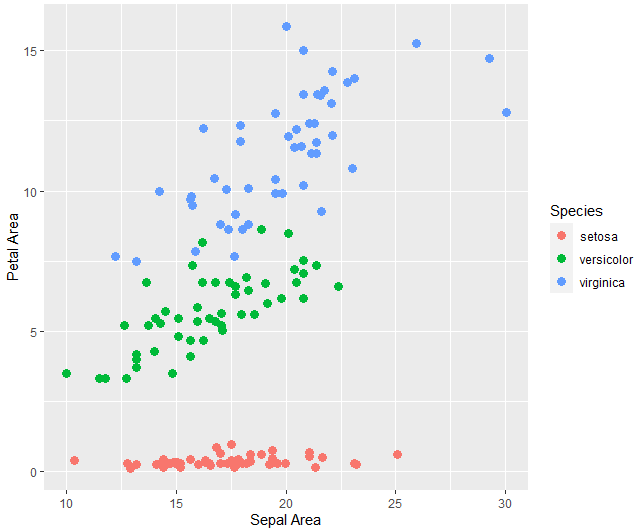
\includegraphics[width=250pt]{chapters/ch-r/figures/qplot_demo.png}
	\caption{A demonstration of \texttt{qplot}.} \label{ch:r1:fig:qplot_demo}
\end{figure}

As a recap, the \verb|mortgage_price| data frame created previously can be visualized as follows. Figures \ref{ch:r1:fig:mortgage_demo1} and \ref{ch:r1:fig:mortgage_demo2} can be obtained.
\begin{lstlisting}
library(ggplot2)
rm(list=ls())
# create data frame
vec_region <-  rep(c("CBD","City","Suburbs"),each = 100)
vec_size_cbd <- rnorm(100, 75, 10)
vec_size_city <- rnorm(100, 100, 15)
vec_size_suburbs <- rnorm(100, 150, 25)
vec_size = c(vec_size_cbd, vec_size_city, vec_size_suburbs)
vec_price_cbd <- vec_size_cbd*rnorm(100, 12500, 2500)
vec_price_city <- vec_size_city*rnorm(100, 7500, 1000)
vec_price_suburbs <- vec_size_suburbs*rnorm(100, 5000, 1000)
vec_price <- c(vec_price_cbd, vec_price_city, vec_price_suburbs)
mortgage_price <- data.frame(Region = vec_region, Size = vec_size, Price = vec_price)
rm(vec_region, vec_size_cbd, vec_size_city, vec_size_suburbs, vec_size, vec_price_cbd, vec_price_city, vec_price_suburbs, vec_price)
# processing
mortgage_price$Price.Unit <- mortgage_price$Price / mortgage_price$Size
# plot
qplot(data=mortgage_price, x=Size, y=Price, color=Region, geom=c("point", "smooth"))
qplot(data=mortgage_price, x=Region, y=Price.Unit, geom="boxplot")
\end{lstlisting}

\begin{figure}
	\centering
	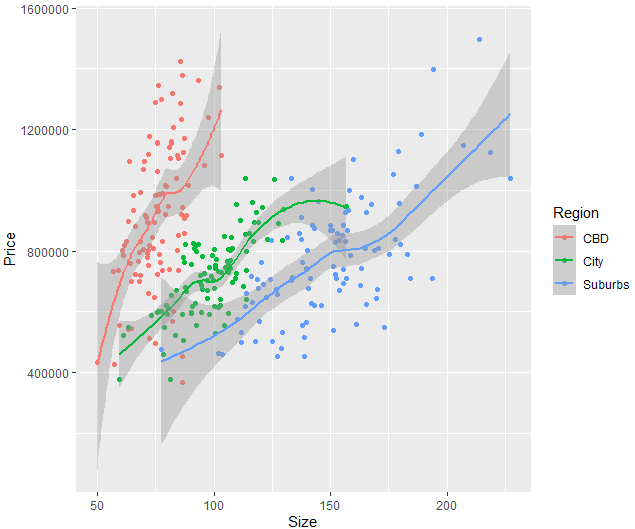
\includegraphics[width=250pt]{chapters/ch-r/figures/mortgage_demo1.png}
	\caption{A demonstration of \texttt{qplot} on mortgage price data frame.} \label{ch:r1:fig:mortgage_demo1}
\end{figure}

\begin{figure}
	\centering
	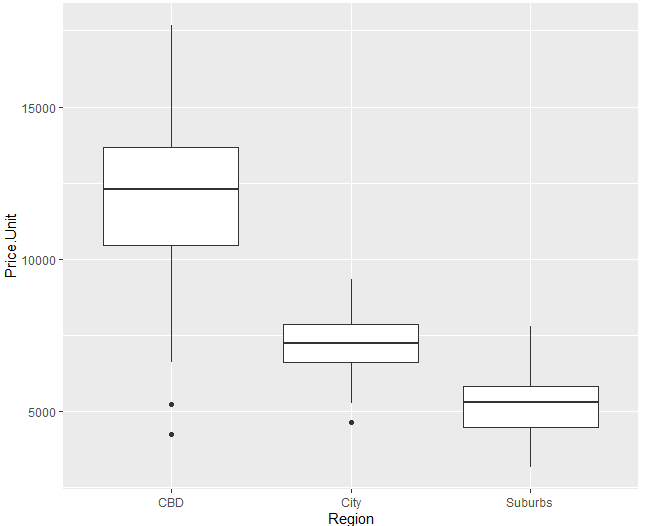
\includegraphics[width=250pt]{chapters/ch-r/figures/mortgage_demo2.png}
	\caption{A second demonstration of \texttt{qplot} on mortgage price data frame.} \label{ch:r1:fig:mortgage_demo2}
\end{figure}

\section{Advanced Data Visualizations Using \texttt{ggplot()}} \label{ch:r1:sec:ggplot}

Function \verb|ggplot()| is the main data visualization tool in \verb|ggolot2| package. It provides very flexible features for data plotting.

\subsection{Grammar of Graphics}

As proposed by Leland Wilkinson's Grammar of Graphics, a chart shall contain multiple independent and reusable layers including
\begin{itemize}
  \item Data. Original data.
  \item Aesthetics. How data is mapped to the graph, for example, by dots, curves, color blocks or lines/bars of different length.
  \item Geometries. The color or shape of each element in the graph.
  \item Statistics. Information derived from the data.
  \item Facets. Subplots of different data sets, and how they are aligned and compared.
  \item Coordinates. The meaning and range of axis.
  \item Theme. Titles, labels, legends, etc.
\end{itemize}
A demonstrative Fig. \ref{ch:r1:fig:chart_layer} is given to illustrate the different layers in a chart.

\begin{figure}
	\centering
	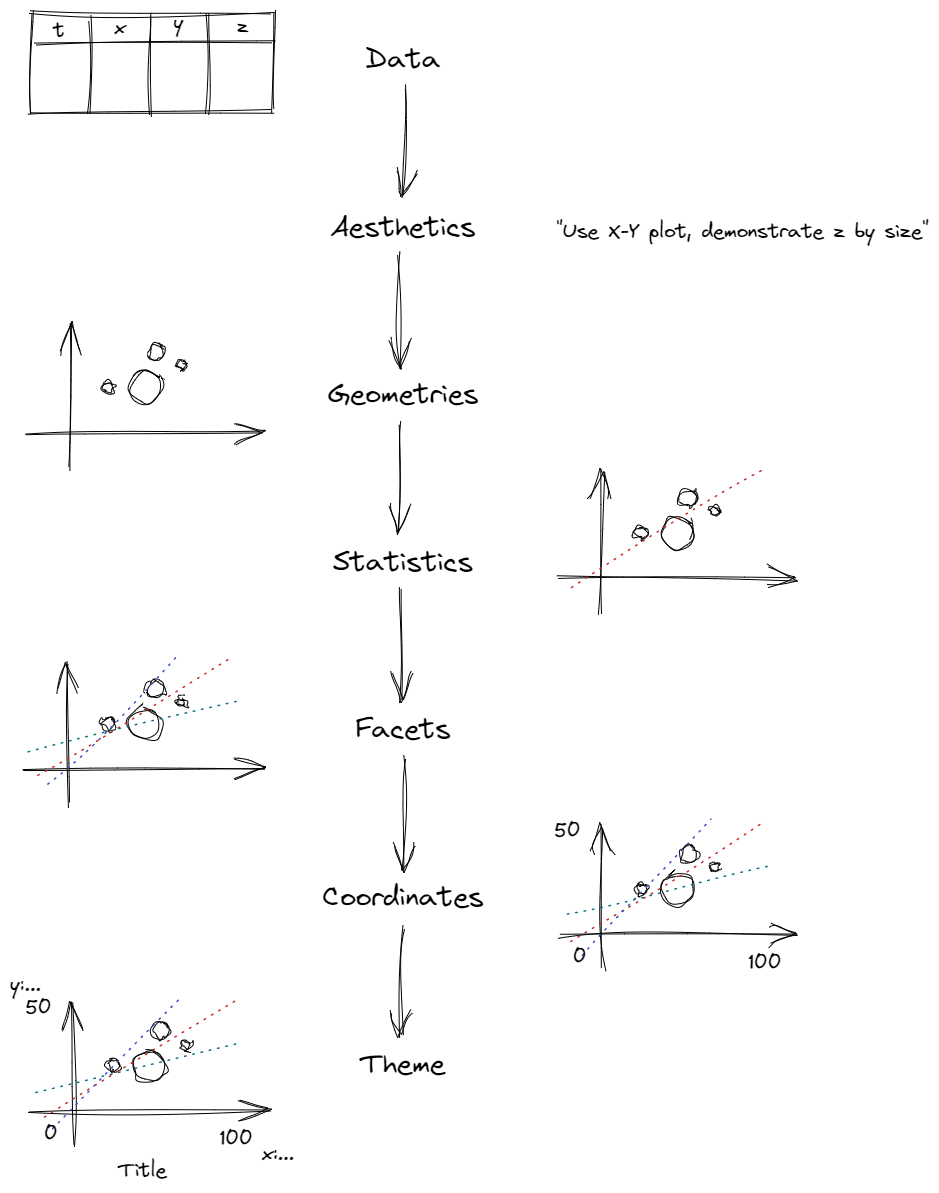
\includegraphics[width=250pt]{chapters/ch-r/figures/chart_layer.png}
	\caption{Multiple layers in chart design.} \label{ch:r1:fig:chart_layer}
\end{figure}

\subsection{Data, Aesthetics and Geometries Layers}

Function \verb|ggplot()| is a very good practice of implementing the above chart design and plotting philosophy. A simple example for \verb|ggplot()|, just for quick demonstration purpose, is given below.
\begin{lstlisting}
p <- ggplot(data=<df>, aes(x=<column>, y=<column>, color=<column>, size=<column>))
p <- p + geom_point()
p
\end{lstlisting}
where \verb|aes()| is used to build mappings in the aesthetics.

An interesting fact when using \verb|ggplot()| is that, when adding a layer to the chat, the layer is literally added to \verb|ggplot()|. In the program, this step by step build up an object, where \verb|ggplot()| provides the most basic layers. Therefore, the above simple example is equivalent to
\begin{lstlisting}
p <- ggplot(data=<df>, aes(x=<column>, y=<column>, color=<column>, size=<column>))
p + geom_point()
p + geom_line() # another selection of geometries choice
p + geom_line() + geom_point() # overlying both geometries choices
p + geom_point(aes(size=<another-column>)) # overwrite aesthetics settings.
\end{lstlisting}
and the added layers are able to inherit the aesthetics settings, if it is not overwritten. And speaking of overwriting, even the x and y axis can be overwritten. The displaying name of the labels can be overwritten by stack \verb|xlab("")| and \verb|ylab("")| into the chart.

Function \verb|ggplot()| provides many choices for geometries. The most commonly used ones are summarized in Table \ref{ch:r1:tab:geoms}.
\begin{table}
  \centering \caption{Commonly used commands for data frame exploration.}\label{ch:r1:tab:geoms}
  \begin{tabularx}{\textwidth}{lX}
    \hline
    \textbf{Geom} & \textbf{Description} \\ \hline
    \verb|geom_point()|   & Scatter plots and dot plots. \\
    \verb|geom_line()|    & Line plots.   \\
    \verb|geom_bar()|     & Bar plots. \\
    \verb|geom_histogram()| & Histograms. \\
    \verb|geom_boxplot()| & Box plots. \\
    \verb|geom_violin()| & Violin plots.\\
    \verb|geom_density()| & Density plots.\\
    \verb|geom_density2d()| & 2-dimensional Density plots.\\
    \verb|geom_text()| & Text Annotation.\\
    \verb|geom_label()| & Label on the observations.\\ \hline
    \end{tabularx}
\end{table}

\subsection{Statistics Layers}

Similar to the case of geometries layers, statistics layers can also be stacked to \verb|ggplot()|. As introduced earlier, statistics layers are often ``add-on'' layers that derives statistical features from the data to provide additional insights. Many functions in Table \ref{ch:r1:tab:geoms} are statistics related. More details are given below.

Consider using \verb|geom_boxplot()| to visualize the \verb|mortgage_price| data frame that was used in the previous section. Examples are given below.
\begin{lstlisting}
library(ggplot2)
# create data frame
vec_region <-  rep(c("CBD","City","Suburbs"), each = 100)
vec_size_cbd <- rnorm(100, 75, 10)
vec_size_city <- rnorm(100, 100, 15)
vec_size_suburbs <- rnorm(100, 150, 25)
vec_size = c(vec_size_cbd, vec_size_city, vec_size_suburbs)
vec_price_cbd <- vec_size_cbd*rnorm(100, 12500, 2500)
vec_price_city <- vec_size_city*rnorm(100, 7500, 1000)
vec_price_suburbs <- vec_size_suburbs*rnorm(100, 5000, 1000)
vec_price <- c(vec_price_cbd, vec_price_city, vec_price_suburbs)
mortgage_price <- data.frame(Region = vec_region, Size = vec_size, Price = vec_price)
rm(vec_region, vec_size_cbd, vec_size_city, vec_size_suburbs, vec_size, vec_price_cbd, vec_price_city, vec_price_suburbs, vec_price)
# processing
mortgage_price$Price.Unit <- mortgage_price$Price / mortgage_price$Size
# plot
p <- ggplot(data=mortgage_price, aes(x=Region, y=Price.Unit, color=Region)) + ggtitle("Mortgage uprice per area VS region") + xlab("Region") + ylab("Price per area")
p + geom_boxplot() + geom_jitter(aes(size=Size, color=Region), alpha=0.25)
\end{lstlisting}
and the result is shown in Fig. \ref{ch:r1:fig:mortgage_barplot_demo}.
\begin{figure}
	\centering
	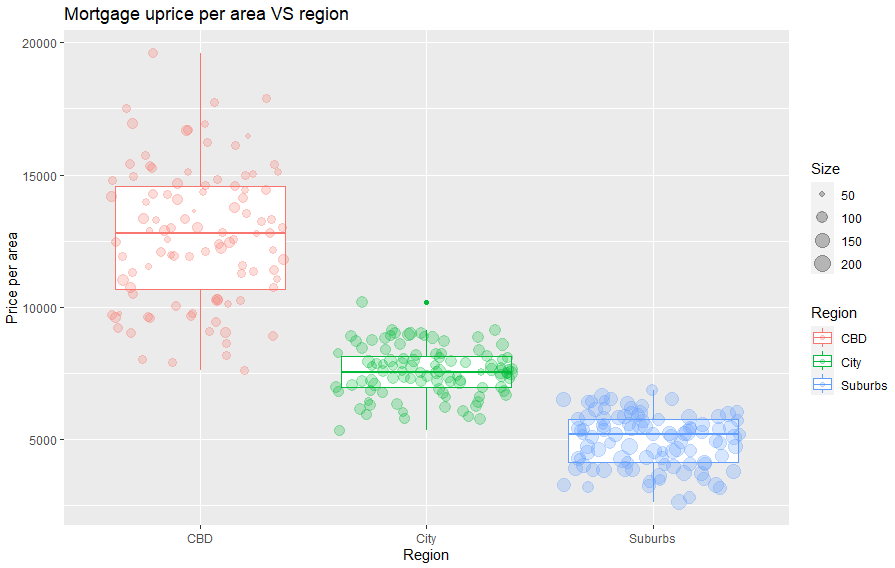
\includegraphics[width=250pt]{chapters/ch-r/figures/mortgage_barplot_demo.png}
	\caption{An example of box plot of the mortgage price data frame using \texttt{ggplot()} and \texttt{geom_boxplot()}.} \label{ch:r1:fig:mortgage_barplot_demo}
\end{figure}
Notice that \verb|ggtitle()|, \verb|xlab()|, \verb|ylab()|, \verb|alpha| are used in the plot. They are self-explanatory. A new geometry \verb|geom_jitter()| is used, which works similarly with \verb|geom_point()| except the additional vibration in the horizontal axis which makes the points clearer to see.

Function \verb|geom_smooth()| is widely used for curve fitting. An example is given below.
\begin{lstlisting}
library(ggplot2)
# generate data
t <- 1:500
var1 <- 1.5*t + rnorm(500, 0, 100)
var2 <- 0.5*t + rnorm(500, 200, 10) + t^1.3*rnorm(500, 0, 0.1)
df <- data.frame(t=t, x=var1, y=var2)
# plot data
p <- ggplot(data=df) +
ggtitle("Plot of x and y VS t.") +
xlab("t") +
ylab("x and y") +
geom_point(aes(x=t, y=x), color="blue", shape=1, size=1.5) +
geom_smooth(aes(x=t, y=x), color="blue") +
geom_point(aes(x=t, y=y), color="red", shape=2, size=1.5) +
geom_smooth(aes(x=t, y=y), color="red")
p
\end{lstlisting}
Do note that aesthetics needs to be given to \verb|geom_smooth()| in the above example. This is because aesthetics is not given in the base \verb|ggolot()|. Notice that \verb|geom_smooth()| can inherit aesthetics from the previous \verb|ggplot()|, but not from the previous \verb|geom_point()|. The plot is given by Fig. \ref{ch:r1:fig:geom_smooth_demo}.
\begin{figure}
	\centering
	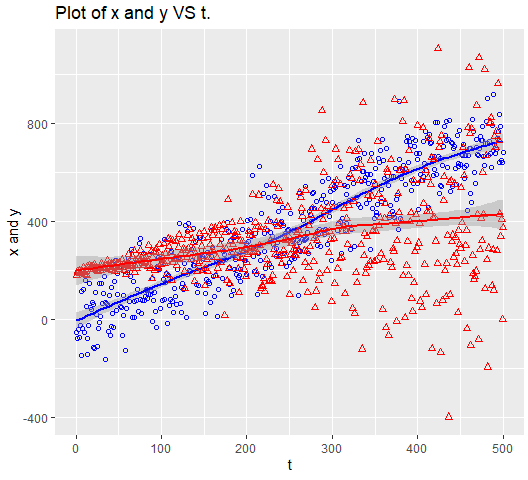
\includegraphics[width=250pt]{chapters/ch-r/figures/geom_smooth_demo.png}
	\caption{An example of using \texttt{geom_smooth()} for scatter point fitting.} \label{ch:r1:fig:geom_smooth_demo}
\end{figure}

More functions similar to \verb|geom_smooth()| are summarized in Table \ref{ch:r1:tab:linefit}.
\begin{table}
	\centering \caption{Functions that fit smooth lines to scatter points.}\label{ch:r1:tab:linefit}
	\begin{tabularx}{\textwidth}{lX}
	\hline
	Function & Description \\ \hline
	\verb|loess()| & Non-parametric method for fitting a smooth line to a scatter plot using locally weighted regression algorithm.\\
	\verb|smooth.spline()| & Fits a smoothing spline to the data, which is a type of regression spline where the degree of smoothing is chosen automatically by cross-validation.\\
	\verb|lm()| & Linear Model, fits a linear relationship between independent and dependent variables by minimizing the residuals between the data points and the line.\\
	\verb|glm()| & Generalized Linear Model, similar to linear model, but it allows different distribution of error other than normal.\\
	\verb|gam()| & Generalized Additive Model, it is similar to GLM, but it allows non-parametric smooth functions to be added to the linear predictor.\\
	\verb|geom_smooth()| & A function in ggplot2 that is used to add a smooth line to a scatter plot, it uses method = "loess" by default but also allow to use other smoothing method like lm, gam etc.\\
	\hline
	\end{tabularx}
\end{table}

\subsection{Facets Layers}

The facets layer allows subplot of data. Consider the following example, where the distribution of mortgage price is studied using histogram. The following code can be used to plot the result in a single plot without the facets layer. The plot is given in Fig. \ref{ch:r1:fig:mortgage_histogram_demo}.
\begin{lstlisting}
library(ggplot2)
# create data frame
Region = rep(c("CBD","City","Suburbs"), each = 500)
vec_size =  list(vec_size_cbd = rnorm(500, 75, 10), vec_size_city = rnorm(500, 100, 15), vec_size_suburbs = rnorm(500, 150, 25))
vec_price = list(vec_price_cbd = vec_size$vec_size_cbd*rnorm(500, 12500, 2500),
                 vec_price_city = vec_size$vec_size_city*rnorm(500, 7500, 1000),
                 vec_price_suburbs = vec_size$vec_size_suburbs*rnorm(500, 5000, 1000))
mortgage_price <- data.frame(Region = Region,
                             Size = unlist(vec_size),
                             Price = unlist(vec_price))
mortgage_price$Region <- as.factor(mortgage_price$Region)
mortgage_price$Price.Unit <- mortgage_price$Price / mortgage_price$Size
# plot data
p <- ggplot(data=mortgage_price, aes(x=Price.Unit))
p + geom_histogram(aes(fill=Region), bins=50, color="black", alpha=0.5, position="identity") +
  ggtitle("Mortgage price per unit area in different regions.") +
  xlab("Price per unit area") +
  ylab("Number of house")
\end{lstlisting}

\begin{figure}
	\centering
	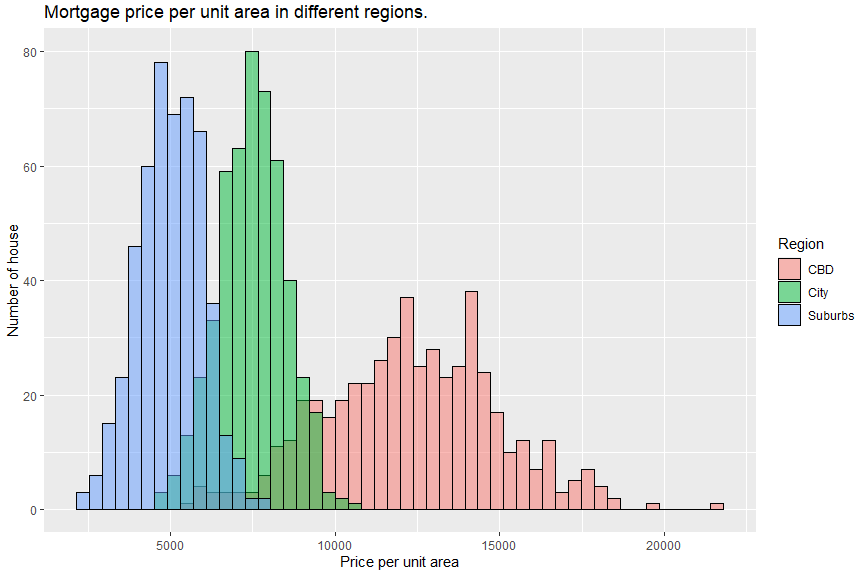
\includegraphics[width=250pt]{chapters/ch-r/figures/mortgage_histogram_demo.png}
	\caption{An example of histogram plot of house price per unit area in different regions in a single plot.} \label{ch:r1:fig:mortgage_histogram_demo}
\end{figure}

To use facets layer, revise the code as follows. Notice that \verb|facet_grid()| is added to the plot, and its input \verb|<column>~.| or \verb|.~<column>| (it is okay to use \verb|<column1>~<column2>| as well) decide the design of the subplots (how to arrange the rows and columns of the subplots).
\begin{lstlisting}
library(ggplot2)
# create data frame
Region = rep(c("CBD","City","Suburbs"), each = 500)
vec_size =  list(vec_size_cbd = rnorm(500, 75, 10),
                 vec_size_city = rnorm(500, 100, 15),
                 vec_size_suburbs = rnorm(500, 150, 25))
vec_price = list(vec_price_cbd = vec_size$vec_size_cbd*rnorm(500, 12500, 2500),
                 vec_price_city = vec_size$vec_size_city*rnorm(500, 7500, 1000),
                 vec_price_suburbs = vec_size$vec_size_suburbs*rnorm(500, 5000, 1000))
mortgage_price <- data.frame(Region = Region,
                             Size = unlist(vec_size),
                             Price = unlist(vec_price))
mortgage_price$Region <- as.factor(mortgage_price$Region)
mortgage_price$Price.Unit <- mortgage_price$Price / mortgage_price$Size
# plot data
p <- ggplot(data=mortgage_price, aes(x=Price.Unit))
p <- p + geom_histogram(aes(fill=Region), bins=50, color="black", alpha=0.5, position="identity") +
  ggtitle("Mortgage price per unit area in different regions.") +
  xlab("Price per unit area") +
  ylab("Number of house")
p
p + facet_grid(Region~.) # put subplots for different regions in rows
p + facet_grid(.~Region) # put subplots for different regions in columns
\end{lstlisting}

The results are given in Figs. \ref{ch:r1:fig:mortgage_histogram_demo_f1} and \ref{ch:r1:fig:mortgage_histogram_demo_f2}, depending on the subplot designs.

\begin{figure}
	\centering
	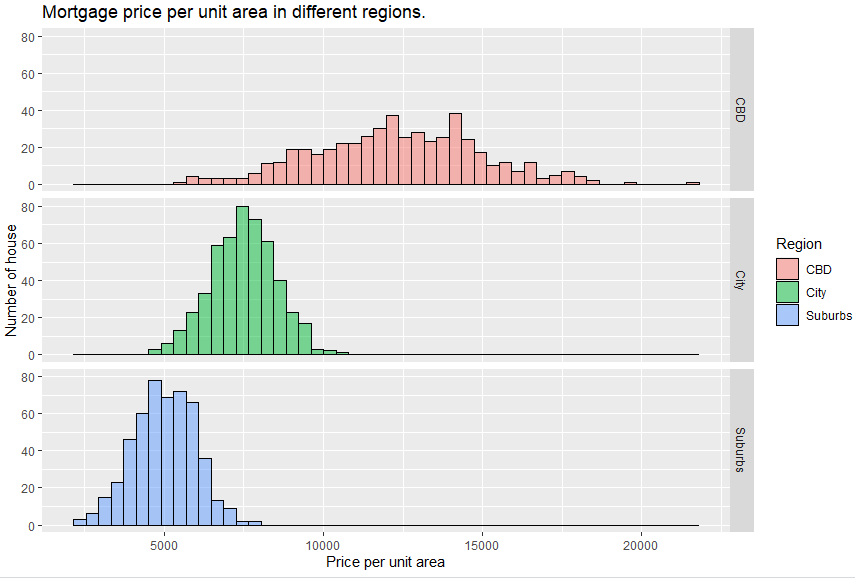
\includegraphics[width=250pt]{chapters/ch-r/figures/mortgage_histogram_demo_f1.png}
	\caption{Use facets to plot the histogram of price per unit are of the house in different regions (subplots in rows).} \label{ch:r1:fig:mortgage_histogram_demo_f1}
\end{figure}

\begin{figure}
	\centering
	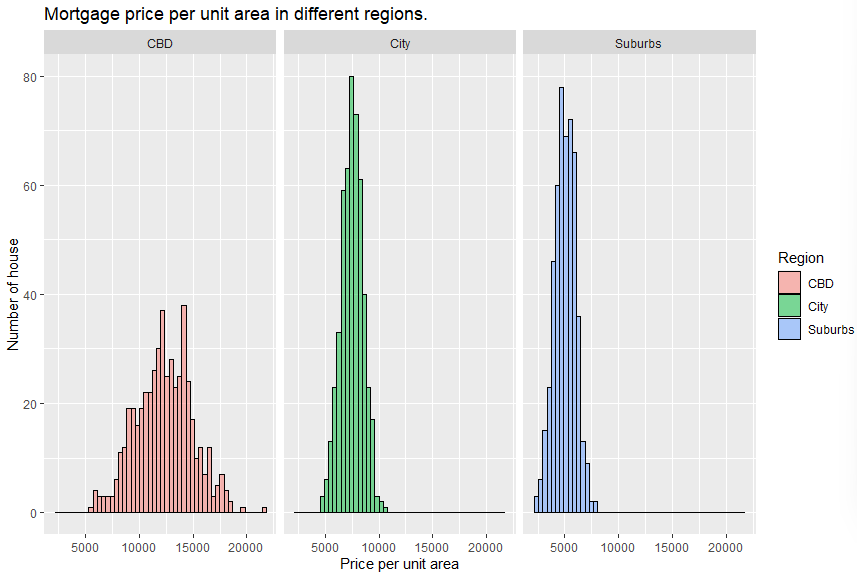
\includegraphics[width=250pt]{chapters/ch-r/figures/mortgage_histogram_demo_f2.png}
	\caption{Use facets to plot the histogram of price per unit are of the house in different regions (subplots in columns).} \label{ch:r1:fig:mortgage_histogram_demo_f2}
\end{figure}

\subsection{Coordinates Layers}

Coordinate control is important. The coordinate layer allows setting limits to the axis and zooming in to the chart. An example of adding coordinates layers to a plot is given as follows. The same mortgage price data frame is used for illustration.
\begin{lstlisting}
library(ggplot2)
# create data frame
Region = rep(c("CBD","City","Suburbs"), each = 500)
vec_size =  list(vec_size_cbd = rnorm(500, 75, 10),
                 vec_size_city = rnorm(500, 100, 15),
                 vec_size_suburbs = rnorm(500, 150, 25))
vec_price = list(vec_price_cbd = vec_size$vec_size_cbd*rnorm(500, 12500, 2500),
                 vec_price_city = vec_size$vec_size_city*rnorm(500, 7500, 1000),
                 vec_price_suburbs = vec_size$vec_size_suburbs*rnorm(500, 5000, 1000))
mortgage_price <- data.frame(Region = Region,
                             Size = unlist(vec_size),
                             Price = unlist(vec_price))
mortgage_price$Region <- as.factor(mortgage_price$Region)
mortgage_price$Price.Unit <- mortgage_price$Price / mortgage_price$Size
# plot data
p <- ggplot(data=mortgage_price, aes(x=Size, y=Price))
p <- p + geom_point(aes(color=Region))
p + xlim(50, 200) + ylim(400000, 1200000) # first chart
p + coord_cartesian(xlim=c(50, 200), ylim = c(400000, 1200000)) # second chart
\end{lstlisting}
where notice that two charts are generated. The first chart using \verb|xlim()|, \verb|ylim| removes all samples outside the boundary from the chart. While in the second chart using \verb|coord_cartesian()|, all samples preserves and the chart zooms in towards the boundary. The results are given in Figs. \ref{ch:r1:fig:coordinate_demo1} and \ref{ch:r1:fig:coordinate_demo2}, respectively. The difference can be observed near the boundary.

\begin{figure}
	\centering
	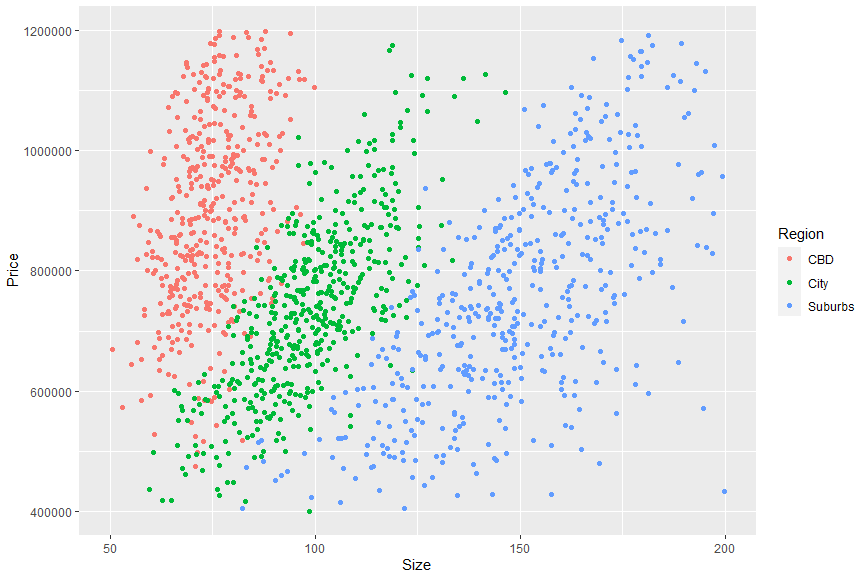
\includegraphics[width=250pt]{chapters/ch-r/figures/coordinate_demo1.png}
	\caption{Add coordinates layer using \texttt{xlim()} and \texttt{ylim()}.} \label{ch:r1:fig:coordinate_demo1}
\end{figure}

\begin{figure}
	\centering
	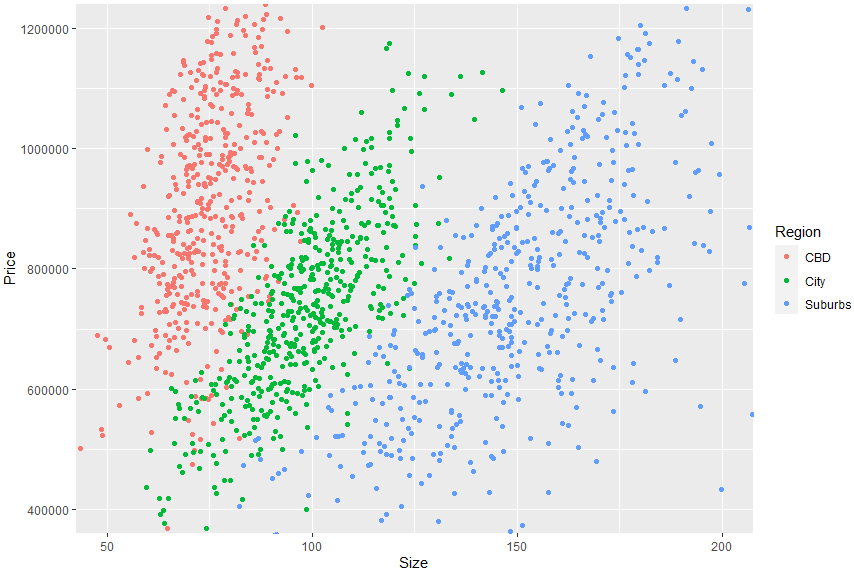
\includegraphics[width=250pt]{chapters/ch-r/figures/coordinate_demo2.png}
	\caption{Add coordinates layer using \texttt{coord_cartesian()}.} \label{ch:r1:fig:coordinate_demo2}
\end{figure}

\subsection{Themes Layers}

Theme layers mainly refer to titles, labels, and other comments on the chart that help with understanding the content of the chart. As already demonstrated in previous examples, use \verb|xlab()|, \verb|ylab()| to add labels, \verb|ggtitle()| to add title.

Use \verb|theme()| to change the themes of the labels. An example is given below.
\begin{lstlisting}
library(ggplot2)
# create data frame
Region = rep(c("CBD","City","Suburbs"), each = 500)
vec_size =  list(vec_size_cbd = rnorm(500, 75, 10), vec_size_city = rnorm(500, 100, 15), vec_size_suburbs = rnorm(500, 150, 25))
vec_price = list(vec_price_cbd = vec_size$vec_size_cbd*rnorm(500, 12500, 2500),
                 vec_price_city = vec_size$vec_size_city*rnorm(500, 7500, 1000),
                 vec_price_suburbs = vec_size$vec_size_suburbs*rnorm(500, 5000, 1000))
mortgage_price <- data.frame(Region = Region,
                             Size = unlist(vec_size),
                             Price = unlist(vec_price))
mortgage_price$Region <- as.factor(mortgage_price$Region)
mortgage_price$Price.Unit <- mortgage_price$Price / mortgage_price$Size
# plot data
p <- ggplot(data=mortgage_price, aes(x=Price.Unit))
p <- p + geom_histogram(aes(fill=Region), bins=50, color="black", alpha=0.5, position="identity")
p + ggtitle("Mortgage price per unit area in different regions.") +
  xlab("Price per unit area") +
  ylab("Number of house") +
  theme(axis.title.x = element_text(color = "DarkGreen", size=15),
        axis.title.y = element_text(color = "DarkRed", size=15),
        axis.text.x = element_text(size=10),
        axis.text.y = element_text(size=10),
        legend.title = element_text(size=10),
        legend.text = element_text(size=8),
        legend.position = c(1,1), # right top corner of chart
        legend.justification = c(1,1), # legend align point
        plot.title = element_text(color = "DarkBlue", size = 15)
  )
\end{lstlisting}

The resulted chart is given in Fig. \ref{ch:r1:fig:mortgage_histogram_theme}. Compare it with Fig. \ref{ch:r1:fig:mortgage_histogram_demo} to see the differences by applying \verb|theme()| in the themes layer.
\begin{figure}
	\centering
	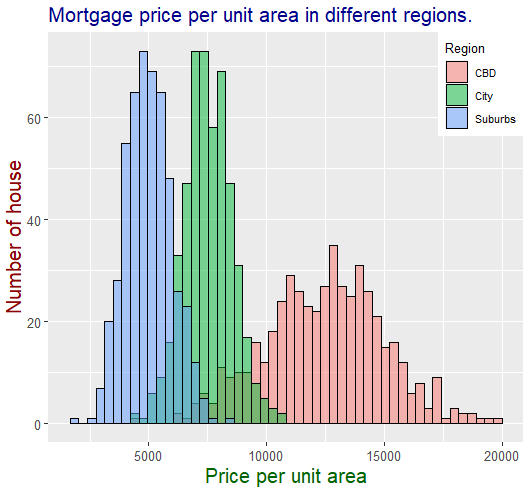
\includegraphics[width=250pt]{chapters/ch-r/figures/mortgage_histogram_theme.png}
	\caption{Mortgage price chart with theme.} \label{ch:r1:fig:mortgage_histogram_theme}
\end{figure}

